% $Header$

\documentclass{beamer}
%\documentclass[handout]{beamer}

\usepackage{amsmath,amssymb,latexsym,eucal,amsthm,graphicx,xcolor}
%%%%%%%%%%%%%%%%%%%%%%%%%%%%%%%%%%%%%%%%%%%%%
% Common Set Theory Constructs
%%%%%%%%%%%%%%%%%%%%%%%%%%%%%%%%%%%%%%%%%%%%%

\newcommand{\setof}[2]{\left\{ \, #1 \, \left| \, #2 \, \right.\right\}}
\newcommand{\lsetof}[2]{\left\{\left. \, #1 \, \right| \, #2 \,  \right\}}
\newcommand{\bigsetof}[2]{\bigl\{ \, #1 \, \bigm | \, #2 \,\bigr\}}
\newcommand{\Bigsetof}[2]{\Bigl\{ \, #1 \, \Bigm | \, #2 \,\Bigr\}}
\newcommand{\biggsetof}[2]{\biggl\{ \, #1 \, \biggm | \, #2 \,\biggr\}}
\newcommand{\Biggsetof}[2]{\Biggl\{ \, #1 \, \Biggm | \, #2 \,\Biggr\}}
\newcommand{\dotsetof}[2]{\left\{ \, #1 \, : \, #2 \, \right\}}
\newcommand{\bigdotsetof}[2]{\bigl\{ \, #1 \, : \, #2 \,\bigr\}}
\newcommand{\Bigdotsetof}[2]{\Bigl\{ \, #1 \, \Bigm : \, #2 \,\Bigr\}}
\newcommand{\biggdotsetof}[2]{\biggl\{ \, #1 \, \biggm : \, #2 \,\biggr\}}
\newcommand{\Biggdotsetof}[2]{\Biggl\{ \, #1 \, \Biggm : \, #2 \,\Biggr\}}
\newcommand{\sequence}[2]{\left\langle \, #1 \,\left| \, #2 \, \right. \right\rangle}
\newcommand{\lsequence}[2]{\left\langle\left. \, #1 \, \right| \,#2 \,  \right\rangle}
\newcommand{\bigsequence}[2]{\bigl\langle \,#1 \, \bigm | \, #2 \, \bigr\rangle}
\newcommand{\Bigsequence}[2]{\Bigl\langle \,#1 \, \Bigm | \, #2 \, \Bigr\rangle}
\newcommand{\biggsequence}[2]{\biggl\langle \,#1 \, \biggm | \, #2 \, \biggr\rangle}
\newcommand{\Biggsequence}[2]{\Biggl\langle \,#1 \, \Biggm | \, #2 \, \Biggr\rangle}
\newcommand{\singleton}[1]{\left\{#1\right\}}
\newcommand{\angles}[1]{\left\langle #1 \right\rangle}
\newcommand{\bigangles}[1]{\bigl\langle #1 \bigr\rangle}
\newcommand{\Bigangles}[1]{\Bigl\langle #1 \Bigr\rangle}
\newcommand{\biggangles}[1]{\biggl\langle #1 \biggr\rangle}
\newcommand{\Biggangles}[1]{\Biggl\langle #1 \Biggr\rangle}


\newcommand{\force}[1]{\Vert\!\underset{\!\!\!\!\!#1}{\!\!\!\relbar\!\!\!%
\relbar\!\!\relbar\!\!\relbar\!\!\!\relbar\!\!\relbar\!\!\relbar\!\!\!%
\relbar\!\!\relbar\!\!\relbar}}
\newcommand{\longforce}[1]{\Vert\!\underset{\!\!\!\!\!#1}{\!\!\!\relbar\!\!\!%
\relbar\!\!\relbar\!\!\relbar\!\!\!\relbar\!\!\relbar\!\!\relbar\!\!\!%
\relbar\!\!\relbar\!\!\relbar\!\!\relbar\!\!\relbar\!\!\relbar\!\!\relbar\!\!\relbar}}
\newcommand{\nforce}[1]{\Vert\!\underset{\!\!\!\!\!#1}{\!\!\!\relbar\!\!\!%
\relbar\!\!\relbar\!\!\relbar\!\!\!\relbar\!\!\relbar\!\!\relbar\!\!\!%
\relbar\!\!\not\relbar\!\!\relbar}}
\newcommand{\forcein}[2]{\overset{#2}{\Vert\underset{\!\!\!\!\!#1}%
{\!\!\!\relbar\!\!\!\relbar\!\!\relbar\!\!\relbar\!\!\!\relbar\!\!\relbar\!%
\!\relbar\!\!\!\relbar\!\!\relbar\!\!\relbar\!\!\relbar\!\!\!\relbar\!\!%
\relbar\!\!\relbar}}}

\newcommand{\pre}[2]{{}^{#2}{#1}}

\newcommand{\restr}{\!\!\upharpoonright\!}

%%%%%%%%%%%%%%%%%%%%%%%%%%%%%%%%%%%%%%%%%%%%%
% Set-Theoretic Connectives
%%%%%%%%%%%%%%%%%%%%%%%%%%%%%%%%%%%%%%%%%%%%%

\newcommand{\intersect}{\cap}
\newcommand{\union}{\cup}
\newcommand{\Intersection}[1]{\bigcap\limits_{#1}}
\newcommand{\Union}[1]{\bigcup\limits_{#1}}
\newcommand{\adjoin}{{}^\frown}
\newcommand{\forces}{\Vdash}

%%%%%%%%%%%%%%%%%%%%%%%%%%%%%%%%%%%%%%%%%%%%%
% Miscellaneous
%%%%%%%%%%%%%%%%%%%%%%%%%%%%%%%%%%%%%%%%%%%%%
\newcommand{\defeq}{=_{\text{def}}}
\newcommand{\Turingleq}{\leq_{\text{T}}}
\newcommand{\Turingless}{<_{\text{T}}}
\newcommand{\lexleq}{\leq_{\text{lex}}}
\newcommand{\lexless}{<_{\text{lex}}}
\newcommand{\Turingequiv}{\equiv_{\text{T}}}
\newcommand{\isomorphic}{\cong}

%%%%%%%%%%%%%%%%%%%%%%%%%%%%%%%%%%%%%%%%%%%%%
% Constants
%%%%%%%%%%%%%%%%%%%%%%%%%%%%%%%%%%%%%%%%%%%%%
\newcommand{\R}{\mathbb{R}}
\renewcommand{\P}{\mathbb{P}}
\newcommand{\Q}{\mathbb{Q}}
\newcommand{\Z}{\mathbb{Z}}
\newcommand{\Zpos}{\Z^{+}}
\newcommand{\Znonneg}{\Z^{\geq 0}}
\newcommand{\C}{\mathbb{C}}
\newcommand{\N}{\mathbb{N}}
\newcommand{\B}{\mathbb{B}}
\newcommand{\Bairespace}{\pre{\omega}{\omega}}
\newcommand{\LofR}{L(\R)}
\newcommand{\JofR}[1]{J_{#1}(\R)}
\newcommand{\SofR}[1]{S_{#1}(\R)}
\newcommand{\JalphaR}{\JofR{\alpha}}
\newcommand{\JbetaR}{\JofR{\beta}}
\newcommand{\JlambdaR}{\JofR{\lambda}}
\newcommand{\SalphaR}{\SofR{\alpha}}
\newcommand{\SbetaR}{\SofR{\beta}}
\newcommand{\Pkl}{\mathcal{P}_{\kappa}(\lambda)}
\DeclareMathOperator{\con}{con}
\DeclareMathOperator{\ORD}{OR}
\DeclareMathOperator{\Ord}{OR}
\DeclareMathOperator{\WO}{WO}
\DeclareMathOperator{\OD}{OD}
\DeclareMathOperator{\HOD}{HOD}
\DeclareMathOperator{\HC}{HC}
\DeclareMathOperator{\WF}{WF}
\DeclareMathOperator{\wfp}{wfp}
\DeclareMathOperator{\HF}{HF}
\newcommand{\One}{I}
\newcommand{\ONE}{I}
\newcommand{\Two}{II}
\newcommand{\TWO}{II}
\newcommand{\Mladder}{M^{\text{ld}}}

%%%%%%%%%%%%%%%%%%%%%%%%%%%%%%%%%%%%%%%%%%%%%
% Commutative Algebra Constants
%%%%%%%%%%%%%%%%%%%%%%%%%%%%%%%%%%%%%%%%%%%%%
\DeclareMathOperator{\dottimes}{\dot{\times}}
\DeclareMathOperator{\dotminus}{\dot{-}}
\DeclareMathOperator{\Spec}{Spec}

%%%%%%%%%%%%%%%%%%%%%%%%%%%%%%%%%%%%%%%%%%%%%
% Theories
%%%%%%%%%%%%%%%%%%%%%%%%%%%%%%%%%%%%%%%%%%%%%
\DeclareMathOperator{\ZFC}{ZFC}
\DeclareMathOperator{\ZF}{ZF}
\DeclareMathOperator{\AD}{AD}
\DeclareMathOperator{\ADR}{AD_{\R}}
\DeclareMathOperator{\KP}{KP}
\DeclareMathOperator{\PD}{PD}
\DeclareMathOperator{\CH}{CH}
\DeclareMathOperator{\GCH}{GCH}
\DeclareMathOperator{\HPC}{HPC} % HOD pair capturing
%%%%%%%%%%%%%%%%%%%%%%%%%%%%%%%%%%%%%%%%%%%%%
% Iteration Trees
%%%%%%%%%%%%%%%%%%%%%%%%%%%%%%%%%%%%%%%%%%%%%

\newcommand{\pred}{\text{-pred}}

%%%%%%%%%%%%%%%%%%%%%%%%%%%%%%%%%%%%%%%%%%%%%%%%
% Operator Names
%%%%%%%%%%%%%%%%%%%%%%%%%%%%%%%%%%%%%%%%%%%%%%%%
\DeclareMathOperator{\Det}{Det}
\DeclareMathOperator{\dom}{dom}
\DeclareMathOperator{\ran}{ran}
\DeclareMathOperator{\range}{ran}
\DeclareMathOperator{\image}{image}
\DeclareMathOperator{\crit}{crit}
\DeclareMathOperator{\card}{card}
\DeclareMathOperator{\cf}{cf}
\DeclareMathOperator{\cof}{cof}
\DeclareMathOperator{\rank}{rank}
\DeclareMathOperator{\ot}{o.t.}
\DeclareMathOperator{\ords}{o}
\DeclareMathOperator{\ro}{r.o.}
\DeclareMathOperator{\rud}{rud}
\DeclareMathOperator{\Powerset}{\mathcal{P}}
\DeclareMathOperator{\length}{lh}
\DeclareMathOperator{\lh}{lh}
\DeclareMathOperator{\limit}{lim}
\DeclareMathOperator{\fld}{fld}
\DeclareMathOperator{\projection}{p}
\DeclareMathOperator{\Ult}{Ult}
\DeclareMathOperator{\ULT}{Ult}
\DeclareMathOperator{\Coll}{Coll}
\DeclareMathOperator{\Col}{Col}
\DeclareMathOperator{\Hull}{Hull}
\DeclareMathOperator*{\dirlim}{dir lim}
\DeclareMathOperator{\Scale}{Scale}
\DeclareMathOperator{\supp}{supp}
\DeclareMathOperator{\trancl}{tran.cl.}
\DeclareMathOperator{\trace}{Tr}
\DeclareMathOperator{\diag}{diag}
\DeclareMathOperator{\spn}{span}
\DeclareMathOperator{\sgn}{sgn}
%%%%%%%%%%%%%%%%%%%%%%%%%%%%%%%%%%%%%%%%%%%%%
% Logical Connectives
%%%%%%%%%%%%%%%%%%%%%%%%%%%%%%%%%%%%%%%%%%%%%
\newcommand{\IImplies}{\Longrightarrow}
\newcommand{\SkipImplies}{\quad\Longrightarrow\quad}
\newcommand{\Ifff}{\Longleftrightarrow}
\newcommand{\iimplies}{\longrightarrow}
\newcommand{\ifff}{\longleftrightarrow}
\newcommand{\Implies}{\Rightarrow}
\newcommand{\Iff}{\Leftrightarrow}
\renewcommand{\implies}{\rightarrow}
\renewcommand{\iff}{\leftrightarrow}
\newcommand{\AND}{\wedge}
\newcommand{\OR}{\vee}
\newcommand{\st}{\text{ s.t. }}
\newcommand{\Or}{\text{ or }}

%%%%%%%%%%%%%%%%%%%%%%%%%%%%%%%%%%%%%%%%%%%%%
% Function Arrows
%%%%%%%%%%%%%%%%%%%%%%%%%%%%%%%%%%%%%%%%%%%%%

\newcommand{\injection}{\xrightarrow{\text{1-1}}}
\newcommand{\surjection}{\xrightarrow{\text{onto}}}
\newcommand{\bijection}{\xrightarrow[\text{onto}]{\text{1-1}}}
\newcommand{\cofmap}{\xrightarrow{\text{cof}}}
\newcommand{\map}{\rightarrow}

%%%%%%%%%%%%%%%%%%%%%%%%%%%%%%%%%%%%%%%%%%%%%
% Mouse Comparison Operators
%%%%%%%%%%%%%%%%%%%%%%%%%%%%%%%%%%%%%%%%%%%%%
\newcommand{\initseg}{\trianglelefteq}
\newcommand{\properseg}{\lhd}
\newcommand{\notinitseg}{\ntrianglelefteq}
\newcommand{\notproperseg}{\ntriangleleft}

%%%%%%%%%%%%%%%%%%%%%%%%%%%%%%%%%%%%%%%%%%%%%
%           calligraphic letters
%%%%%%%%%%%%%%%%%%%%%%%%%%%%%%%%%%%%%%%%%%%%%
\newcommand{\cA}{\mathcal{A}}
\newcommand{\cB}{\mathcal{B}}
\newcommand{\cC}{\mathcal{C}}
\newcommand{\cD}{\mathcal{D}}
\newcommand{\cE}{\mathcal{E}}
\newcommand{\cF}{\mathcal{F}}
\newcommand{\cG}{\mathcal{G}}
\newcommand{\cH}{\mathcal{H}}
\newcommand{\cI}{\mathcal{I}}
\newcommand{\cJ}{\mathcal{J}}
\newcommand{\cK}{\mathcal{K}}
\newcommand{\cL}{\mathcal{L}}
\newcommand{\cM}{\mathcal{M}}
\newcommand{\cN}{\mathcal{N}}
\newcommand{\cO}{\mathcal{O}}
\newcommand{\cP}{\mathcal{P}}
\newcommand{\cQ}{\mathcal{Q}}
\newcommand{\cR}{\mathcal{R}}
\newcommand{\cS}{\mathcal{S}}
\newcommand{\cT}{\mathcal{T}}
\newcommand{\cU}{\mathcal{U}}
\newcommand{\cV}{\mathcal{V}}
\newcommand{\cW}{\mathcal{W}}
\newcommand{\cX}{\mathcal{X}}
\newcommand{\cY}{\mathcal{Y}}
\newcommand{\cZ}{\mathcal{Z}}


%%%%%%%%%%%%%%%%%%%%%%%%%%%%%%%%%%%%%%%%%%%%%
%          Primed Letters
%%%%%%%%%%%%%%%%%%%%%%%%%%%%%%%%%%%%%%%%%%%%%
\newcommand{\aprime}{a^{\prime}}
\newcommand{\bprime}{b^{\prime}}
\newcommand{\cprime}{c^{\prime}}
\newcommand{\dprime}{d^{\prime}}
\newcommand{\eprime}{e^{\prime}}
\newcommand{\fprime}{f^{\prime}}
\newcommand{\gprime}{g^{\prime}}
\newcommand{\hprime}{h^{\prime}}
\newcommand{\iprime}{i^{\prime}}
\newcommand{\jprime}{j^{\prime}}
\newcommand{\kprime}{k^{\prime}}
\newcommand{\lprime}{l^{\prime}}
\newcommand{\mprime}{m^{\prime}}
\newcommand{\nprime}{n^{\prime}}
\newcommand{\oprime}{o^{\prime}}
\newcommand{\pprime}{p^{\prime}}
\newcommand{\qprime}{q^{\prime}}
\newcommand{\rprime}{r^{\prime}}
\newcommand{\sprime}{s^{\prime}}
\newcommand{\tprime}{t^{\prime}}
\newcommand{\uprime}{u^{\prime}}
\newcommand{\vprime}{v^{\prime}}
\newcommand{\wprime}{w^{\prime}}
\newcommand{\xprime}{x^{\prime}}
\newcommand{\yprime}{y^{\prime}}
\newcommand{\zprime}{z^{\prime}}
\newcommand{\Aprime}{A^{\prime}}
\newcommand{\Bprime}{B^{\prime}}
\newcommand{\Cprime}{C^{\prime}}
\newcommand{\Dprime}{D^{\prime}}
\newcommand{\Eprime}{E^{\prime}}
\newcommand{\Fprime}{F^{\prime}}
\newcommand{\Gprime}{G^{\prime}}
\newcommand{\Hprime}{H^{\prime}}
\newcommand{\Iprime}{I^{\prime}}
\newcommand{\Jprime}{J^{\prime}}
\newcommand{\Kprime}{K^{\prime}}
\newcommand{\Lprime}{L^{\prime}}
\newcommand{\Mprime}{M^{\prime}}
\newcommand{\Nprime}{N^{\prime}}
\newcommand{\Oprime}{O^{\prime}}
\newcommand{\Pprime}{P^{\prime}}
\newcommand{\Qprime}{Q^{\prime}}
\newcommand{\Rprime}{R^{\prime}}
\newcommand{\Sprime}{S^{\prime}}
\newcommand{\Tprime}{T^{\prime}}
\newcommand{\Uprime}{U^{\prime}}
\newcommand{\Vprime}{V^{\prime}}
\newcommand{\Wprime}{W^{\prime}}
\newcommand{\Xprime}{X^{\prime}}
\newcommand{\Yprime}{Y^{\prime}}
\newcommand{\Zprime}{Z^{\prime}}
\newcommand{\alphaprime}{\alpha^{\prime}}
\newcommand{\betaprime}{\beta^{\prime}}
\newcommand{\gammaprime}{\gamma^{\prime}}
\newcommand{\Gammaprime}{\Gamma^{\prime}}
\newcommand{\deltaprime}{\delta^{\prime}}
\newcommand{\epsilonprime}{\epsilon^{\prime}}
\newcommand{\kappaprime}{\kappa^{\prime}}
\newcommand{\lambdaprime}{\lambda^{\prime}}
\newcommand{\rhoprime}{\rho^{\prime}}
\newcommand{\Sigmaprime}{\Sigma^{\prime}}
\newcommand{\tauprime}{\tau^{\prime}}
\newcommand{\xiprime}{\xi^{\prime}}
\newcommand{\thetaprime}{\theta^{\prime}}
\newcommand{\Omegaprime}{\Omega^{\prime}}
\newcommand{\cMprime}{\cM^{\prime}}
\newcommand{\cNprime}{\cN^{\prime}}
\newcommand{\cPprime}{\cP^{\prime}}
\newcommand{\cQprime}{\cQ^{\prime}}
\newcommand{\cRprime}{\cR^{\prime}}
\newcommand{\cSprime}{\cS^{\prime}}
\newcommand{\cTprime}{\cT^{\prime}}

%%%%%%%%%%%%%%%%%%%%%%%%%%%%%%%%%%%%%%%%%%%%%
%          bar Letters
%%%%%%%%%%%%%%%%%%%%%%%%%%%%%%%%%%%%%%%%%%%%%
\newcommand{\abar}{\bar{a}}
\newcommand{\bbar}{\bar{b}}
\newcommand{\cbar}{\bar{c}}
\newcommand{\ibar}{\bar{i}}
\newcommand{\jbar}{\bar{j}}
\newcommand{\nbar}{\bar{n}}
\newcommand{\xbar}{\bar{x}}
\newcommand{\ybar}{\bar{y}}
\newcommand{\zbar}{\bar{z}}
\newcommand{\pibar}{\bar{\pi}}
\newcommand{\phibar}{\bar{\varphi}}
\newcommand{\psibar}{\bar{\psi}}
\newcommand{\thetabar}{\bar{\theta}}
\newcommand{\nubar}{\bar{\nu}}

%%%%%%%%%%%%%%%%%%%%%%%%%%%%%%%%%%%%%%%%%%%%%
%          star Letters
%%%%%%%%%%%%%%%%%%%%%%%%%%%%%%%%%%%%%%%%%%%%%
\newcommand{\phistar}{\phi^{*}}
\newcommand{\Mstar}{M^{*}}

%%%%%%%%%%%%%%%%%%%%%%%%%%%%%%%%%%%%%%%%%%%%%
%          dotletters Letters
%%%%%%%%%%%%%%%%%%%%%%%%%%%%%%%%%%%%%%%%%%%%%
\newcommand{\Gdot}{\dot{G}}

%%%%%%%%%%%%%%%%%%%%%%%%%%%%%%%%%%%%%%%%%%%%%
%         check Letters
%%%%%%%%%%%%%%%%%%%%%%%%%%%%%%%%%%%%%%%%%%%%%
\newcommand{\deltacheck}{\check{\delta}}
\newcommand{\gammacheck}{\check{\gamma}}


%%%%%%%%%%%%%%%%%%%%%%%%%%%%%%%%%%%%%%%%%%%%%
%          Formulas
%%%%%%%%%%%%%%%%%%%%%%%%%%%%%%%%%%%%%%%%%%%%%

\newcommand{\formulaphi}{\text{\large $\varphi$}}
\newcommand{\Formulaphi}{\text{\Large $\varphi$}}


%%%%%%%%%%%%%%%%%%%%%%%%%%%%%%%%%%%%%%%%%%%%%
%          Fraktur Letters
%%%%%%%%%%%%%%%%%%%%%%%%%%%%%%%%%%%%%%%%%%%%%

\newcommand{\fa}{\mathfrak{a}}
\newcommand{\fb}{\mathfrak{b}}
\newcommand{\fc}{\mathfrak{c}}
\newcommand{\fk}{\mathfrak{k}}
\newcommand{\fp}{\mathfrak{p}}
\newcommand{\fq}{\mathfrak{q}}
\newcommand{\fr}{\mathfrak{r}}
\newcommand{\fA}{\mathfrak{A}}
\newcommand{\fB}{\mathfrak{B}}
\newcommand{\fC}{\mathfrak{C}}
\newcommand{\fD}{\mathfrak{D}}

%%%%%%%%%%%%%%%%%%%%%%%%%%%%%%%%%%%%%%%%%%%%%
%          Bold Letters
%%%%%%%%%%%%%%%%%%%%%%%%%%%%%%%%%%%%%%%%%%%%%
\newcommand{\ba}{\mathbf{a}}
\newcommand{\bb}{\mathbf{b}}
\newcommand{\bc}{\mathbf{c}}
\newcommand{\bd}{\mathbf{d}}
\newcommand{\be}{\mathbf{e}}
\newcommand{\bu}{\mathbf{u}}
\newcommand{\bv}{\mathbf{v}}
\newcommand{\bw}{\mathbf{w}}
\newcommand{\bx}{\mathbf{x}}
\newcommand{\by}{\mathbf{y}}
\newcommand{\bz}{\mathbf{z}}
\newcommand{\bSigma}{\boldsymbol{\Sigma}}
\newcommand{\bPi}{\boldsymbol{\Pi}}
\newcommand{\bDelta}{\boldsymbol{\Delta}}
\newcommand{\bdelta}{\boldsymbol{\delta}}
\newcommand{\bgamma}{\boldsymbol{\gamma}}
\newcommand{\bGamma}{\boldsymbol{\Gamma}}

%%%%%%%%%%%%%%%%%%%%%%%%%%%%%%%%%%%%%%%%%%%%%
%         Bold numbers
%%%%%%%%%%%%%%%%%%%%%%%%%%%%%%%%%%%%%%%%%%%%%
\newcommand{\bzero}{\mathbf{0}}

%%%%%%%%%%%%%%%%%%%%%%%%%%%%%%%%%%%%%%%%%%%%%
% Projective-Like Pointclasses
%%%%%%%%%%%%%%%%%%%%%%%%%%%%%%%%%%%%%%%%%%%%%
\newcommand{\Sa}[2][\alpha]{\Sigma_{(#1,#2)}}
\newcommand{\Pa}[2][\alpha]{\Pi_{(#1,#2)}}
\newcommand{\Da}[2][\alpha]{\Delta_{(#1,#2)}}
\newcommand{\Aa}[2][\alpha]{A_{(#1,#2)}}
\newcommand{\Ca}[2][\alpha]{C_{(#1,#2)}}
\newcommand{\Qa}[2][\alpha]{Q_{(#1,#2)}}
\newcommand{\da}[2][\alpha]{\delta_{(#1,#2)}}
\newcommand{\leqa}[2][\alpha]{\leq_{(#1,#2)}}
\newcommand{\lessa}[2][\alpha]{<_{(#1,#2)}}
\newcommand{\equiva}[2][\alpha]{\equiv_{(#1,#2)}}


\newcommand{\Sl}[1]{\Sa[\lambda]{#1}}
\newcommand{\Pl}[1]{\Pa[\lambda]{#1}}
\newcommand{\Dl}[1]{\Da[\lambda]{#1}}
\newcommand{\Al}[1]{\Aa[\lambda]{#1}}
\newcommand{\Cl}[1]{\Ca[\lambda]{#1}}
\newcommand{\Ql}[1]{\Qa[\lambda]{#1}}

\newcommand{\San}{\Sa{n}}
\newcommand{\Pan}{\Pa{n}}
\newcommand{\Dan}{\Da{n}}
\newcommand{\Can}{\Ca{n}}
\newcommand{\Qan}{\Qa{n}}
\newcommand{\Aan}{\Aa{n}}
\newcommand{\dan}{\da{n}}
\newcommand{\leqan}{\leqa{n}}
\newcommand{\lessan}{\lessa{n}}
\newcommand{\equivan}{\equiva{n}}

\newcommand{\SigmaOneOmega}{\Sigma^1_{\omega}}
\newcommand{\SigmaOneOmegaPlusOne}{\Sigma^1_{\omega+1}}
\newcommand{\PiOneOmega}{\Pi^1_{\omega}}
\newcommand{\PiOneOmegaPlusOne}{\Pi^1_{\omega+1}}
\newcommand{\DeltaOneOmegaPlusOne}{\Delta^1_{\omega+1}}

%%%%%%%%%%%%%%%%%%%%%%%%%%%%%%%%%%%%%%%%%%%%%
% Linear Algebra
%%%%%%%%%%%%%%%%%%%%%%%%%%%%%%%%%%%%%%%%%%%%%
\newcommand{\transpose}[1]{{#1}^{\text{T}}}
\newcommand{\norm}[1]{\lVert{#1}\rVert}
\newcommand\aug{\fboxsep=-\fboxrule\!\!\!\fbox{\strut}\!\!\!}

%%%%%%%%%%%%%%%%%%%%%%%%%%%%%%%%%%%%%%%%%%%%%
% Number Theory
%%%%%%%%%%%%%%%%%%%%%%%%%%%%%%%%%%%%%%%%%%%%%
\newcommand{\av}[1]{\lvert#1\rvert}
\DeclareMathOperator{\divides}{\mid}
\DeclareMathOperator{\ndivides}{\nmid}
\DeclareMathOperator{\lcm}{lcm}
\DeclareMathOperator{\sign}{sign}
\newcommand{\floor}[1]{\left\lfloor{#1}\right\rfloor}
\DeclareMathOperator{\ConCl}{CC}
\DeclareMathOperator{\ord}{ord}



\graphicspath{{images/}}

\newtheorem*{claim}{claim}
\newtheorem*{observation}{Observation}
\newtheorem*{warning}{Warning}
\newtheorem*{question}{Question}
\newtheorem{remark}[theorem]{Remark}

\newenvironment*{subproof}[1][Proof]
{\begin{proof}[#1]}{\renewcommand{\qedsymbol}{$\diamondsuit$} \end{proof}}

\mode<presentation>
{
  \usetheme{Singapore}
  % or ...

  \setbeamercovered{invisible}
  % or whatever (possibly just delete it)
}


\usepackage[english]{babel}
% or whatever

\usepackage[latin1]{inputenc}
% or whatever

\usepackage{times}
\usepackage[T1]{fontenc}
% Or whatever. Note that the encoding and the font should match. If T1
% does not look nice, try deleting the line with the fontenc.

\title{Lesson 9\\ Gaussian elimination, Part 2}
\subtitle{Math 325, Linear Algebra \\ Spring 2019 \\ SFSU}
\author{Mitch Rudominer}
\date{}



% If you wish to uncover everything in a step-wise fashion, uncomment
% the following command:

\beamerdefaultoverlayspecification{<+->}

\begin{document}

\begin{frame}
  \titlepage
\end{frame}

%%%%%%%%%%%%%%%%%%%%%%%%%%%%%%%%%%%%%%%%%%%%%%%%%%%%%%%%%%%%%%%%%%%%%%%%%

\begin{frame}{Gaussian elimination: The Non-Simple Case}

\begin{itemize}
\item In the last lesson we learned the simple case of Gaussian elimination.
\item We start with a square matrix $A$.
\item After applying a series of row operations we transform $A$
into a new matrix $\Aprime$ that is upper-triangular with non-zeros on the diagonal.
\item This happens when our original matrix $A$ is a square invertible matrix.
\item But what if this is not the case?
\item What if $A$ is not invertible, or not even square?
\item Then we end up with a matrix $\Aprime$ in a slightly more complicated form.
\end{itemize}

\end{frame}


%%%%%%%%%%%%%%%%%%%%%%%%%%%%%%%%%%%%%%%%%%%%%%%%%%%%%%%%%%%%%%%%%%%%%%%%%

\begin{frame}{Row-Echelon Form}

\begin{center}
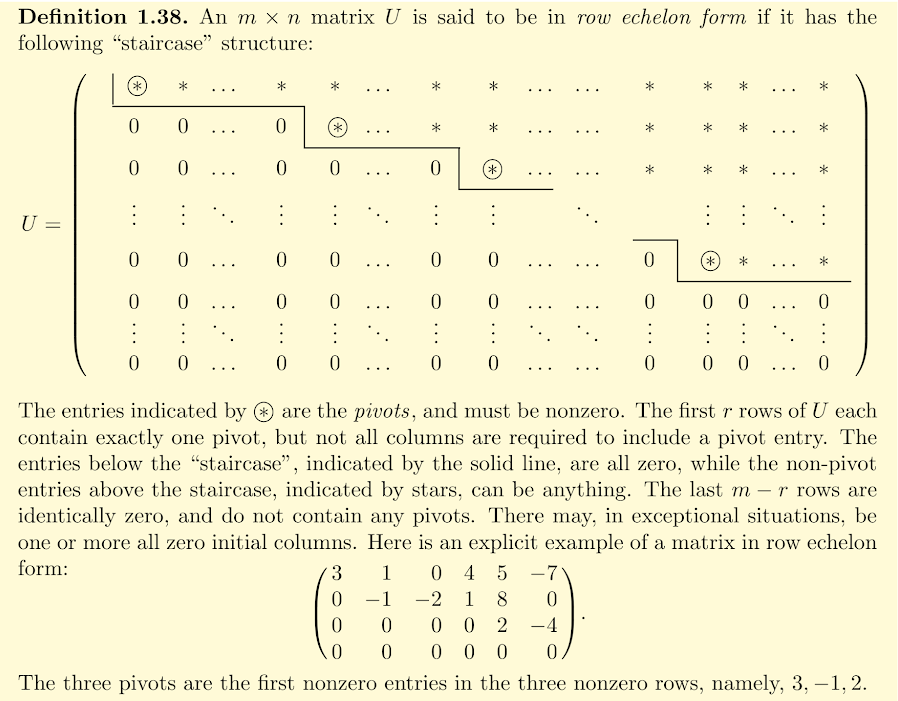
\includegraphics[scale=0.25]{row-echelon-form}
\end{center}

\end{frame}

%%%%%%%%%%%%%%%%%%%%%%%%%%%%%%%%%%%%%%%%%%%%%%%%%%%%%%%%%%%%%%%%%%%%%%%%%

\begin{frame}{Row-Echelon Form}

\begin{itemize}
\item \textbf{Definition.} Let $A = \left(\bv_1 \vert \bv_2 \vert \cdots \vert \bv_n\right)$
be an $m\times n$ matrix with columns $\bv_1,\bv_2,\cdots,\bv_n$.
\item Then $A$ is in \emph{row-echelon form} iff it follows these rules:
\item Let $\bv_f$ be the first non-zero column
\item Then $\bv_f$ has a non-zero in position 1 and zeros
in all other positions.
\item Now for each $i>=f$, if $\bv_i\not=\bzero$, let $k_i$ be the largest index of a non-zero entry in $\bv_i$.
\item Then $k_i<=\max \setof{k_j}{j<i} +1$.
\item If $k_i=\max \setof{k_j}{j<i} +1$ then $\bv_i$ is called a pivot column and the $k_i^{\text{th}}$ element
of $\bv_i$ is called a pivot.
\item Otherwise $k_i<= \max \setof{k_j}{j<i}$ and $\bv_i$ is called a non-pivot column.

\end{itemize}

\end{frame}


%%%%%%%%%%%%%%%%%%%%%%%%%%%%%%%%%%%%%%%%%%%%%%%%%%%%%%%%%%%%%%%%%%%%%%%%%

\begin{frame}{The Pivot Columns}

$
\begin{pmatrix}
\textcolor{red}{\mathbf{3}} & \mathbf{1}                   &  0  & 4 & \mathbf{5}                  & -7 \\
\mathbf{0}                  & \textcolor{red}{\mathbf{-1}} & -2  & 1 & \mathbf{0}                  & 0  \\
\mathbf{0}                  & \mathbf{0}                   &  0  & 0 & \textcolor{red}{\mathbf{2}} & -4 \\
\mathbf{0}                  & \mathbf{0}                   &  0  & 0 & \mathbf{0}                  & 0  \\
\end{pmatrix}
$
\begin{itemize}
\item The bolded columns are called the \emph{pivot} columns. The red entries are the pivots.
\item The pivots must all be non-zero.
\item There must be zeros below the pivots.
\item Above the pivots can be anything.
\item The first pivot is the first entry of the first pivot column.
\item The second pivot is the second entry of the second pivot column. Etc.
\item The non-pivot columns must have zeros below the pivot column immediately to the left.
\end{itemize}

\end{frame}

%%%%%%%%%%%%%%%%%%%%%%%%%%%%%%%%%%%%%%%%%%%%%%%%%%%%%%%%%%%%%%%%%%%%%%%%%

\begin{frame}{Example}

Let
$
A=
\begin{pmatrix}
5 & -2 &  7  & 0 \\
0 & 0  & -1  & 1 \\
0 & 0  &  0  & 3 \\
0 & 0  &  0  & 0 \\
\end{pmatrix}
$
\begin{itemize}
\item Is $A$ in row-echelon form?
\item Yes.
\end{itemize}

\end{frame}

%%%%%%%%%%%%%%%%%%%%%%%%%%%%%%%%%%%%%%%%%%%%%%%%%%%%%%%%%%%%%%%%%%%%%%%%%

\begin{frame}{Example}

Let
$
A=
\begin{pmatrix}
2 & -2 &  0 \\
0 & 5  &  1 \\
0 & 0  &  3 \\
\end{pmatrix}
$
\begin{itemize}
\item Is $A$ in row-echelon form?
\item Yes. $A$ is upper-triangular with nonzeros on the diagonal.
That is a special case of row-echelon form.
\end{itemize}

\end{frame}

%%%%%%%%%%%%%%%%%%%%%%%%%%%%%%%%%%%%%%%%%%%%%%%%%%%%%%%%%%%%%%%%%%%%%%%%%

\begin{frame}{Example}

Let
$
A=
\begin{pmatrix}
0 & -2  &   1 \\
0 &  0  &   0 \\
0 &  0  &   0 \\
\end{pmatrix}
$
\begin{itemize}
\item Is $A$ in row-echelon form?
\item Yes. Row-echelon form is allowed to have zero columns on the left.
\end{itemize}

\end{frame}

%%%%%%%%%%%%%%%%%%%%%%%%%%%%%%%%%%%%%%%%%%%%%%%%%%%%%%%%%%%%%%%%%%%%%%%%%

\begin{frame}{Example}

Let
$
A=
\begin{pmatrix}
2 & -2  &   1 \\
3 &  0  &   0 \\
0 &  0  &   0 \\
\end{pmatrix}
$
\begin{itemize}
\item Is $A$ in row-echelon form?
\item No
\end{itemize}

\end{frame}

%%%%%%%%%%%%%%%%%%%%%%%%%%%%%%%%%%%%%%%%%%%%%%%%%%%%%%%%%%%%%%%%%%%%%%%%%

\begin{frame}{Gaussian elimination}

\begin{itemize}
\item Given any rectangular matrix $A$, we can perform Gaussian elimination on it.
\item This yields another matrix $\Aprime$ of the same size that is in row-echelon form.
\item This is a generalization of the simple case we learned in the previous lesson.
\end{itemize}

\end{frame}


%%%%%%%%%%%%%%%%%%%%%%%%%%%%%%%%%%%%%%%%%%%%%%%%%%%%%%%%%%%%%%%%%%%%%%%%%

\begin{frame}{Gaussian elimination Algorithm by Example}

\begin{itemize}
\item Use Gaussian elimination to bring the following matrix to row-echelon
form.
\item $
\begin{pmatrix}
0 & 0  &   0  &  0   &  1  &  2 \\
0 & 1  &  17  & -11  &  0  &  1  \\
0 & 2  &  34  & -20  &  0  &  0 \\
0 & -1 &  -17   &  6 &  3  &  1 \\
\end{pmatrix}
$
\item First skip any all-zero columns on the left.
\item Start working with the first non-zero column. In our case that is column 2.
\item This will be the first pivot column.
\item We need a non-zero entry in the first position of the first pivot column.
\item Currently we have a 0 in the first position.
\item We have to perform a swap in order to put a nonzero there. (An elementary row operation of type II)
\item Swap rows 1 and 2
\end{itemize}
\end{frame}

%%%%%%%%%%%%%%%%%%%%%%%%%%%%%%%%%%%%%%%%%%%%%%%%%%%%%%%%%%%%%%%%%%%%%%%%%

\begin{frame}{Gaussian elimination Algorithm by Example}

\begin{itemize}
\item $
\begin{pmatrix}
0 & \textbf{1} &  17    & -11   &  0  &  1  \\
0 &         0  &   0    &   0    &  1  &  2 \\
0 &         2  &  34    &  -20  &  0  &  0 \\
0 &        -1  &  -17   &  6    &  3  &  1 \\
\end{pmatrix}
$
\item Now the bolded 1 is our first pivot.
\item Next we use row operations of type I in order to change all of the
entries below the first pivot to zero.
\item Replace row 3 with row 3 minus 2 times row 1
\item $
\begin{pmatrix}
0 & \textbf{1} &  17   & -11  &  0  &  1  \\
0 &         0  &   0   &  0   &  1  &  2 \\
0 &         0  &   0   &  2   &  0  &  -2 \\
0 &        -1  &  -17   &  6   &  3  &  1 \\
\end{pmatrix}
$
\end{itemize}
\end{frame}

%%%%%%%%%%%%%%%%%%%%%%%%%%%%%%%%%%%%%%%%%%%%%%%%%%%%%%%%%%%%%%%%%%%%%%%%%

\begin{frame}{Gaussian elimination Algorithm by Example}

\begin{itemize}
\item $
\begin{pmatrix}
0 & \textbf{1} &  17   & -11  &  0  &  1  \\
0 &         0  &  0    &  0   &  1  &  2 \\
0 &         0  &  0    &  2   &  0  &  -2 \\
0 &        -1  &  -17  &  6   &  3  &  1 \\
\end{pmatrix}
$
\item Replace row 4 with row 4 plus row 1
\item $
\begin{pmatrix}
0 & \textbf{1} &  17   &  -11   &  0  &  1  \\
0 &         0  &   0   &   0    &  1  &  2 \\
0 &         0  &   0   &   2   &  0  &  -2 \\
0 &         0  &   0   &  -5   &  3  &  2 \\
\end{pmatrix}
$
\item Now we need to find the next pivot column. Look for the
next column with a nonzero below the first pivot.
\item Column 3 does not have this.
\item Column 4 does. So column 4 is our next pivot column.
\item But column 4 does not have a nonzero in row 2.
\end{itemize}
\end{frame}

%%%%%%%%%%%%%%%%%%%%%%%%%%%%%%%%%%%%%%%%%%%%%%%%%%%%%%%%%%%%%%%%%%%%%%%%

\begin{frame}{Gaussian elimination Algorithm by Example}

\begin{itemize}
\item $
\begin{pmatrix}
0 & \textbf{1} &  17   &  -11   &  0  &  1   \\
0 &         0  &   0   &   0    &  1  &  2   \\
0 &         0  &   0   &   2   &   0  &  -2  \\
0 &         0  &   0   &  -5   &   3  &  2   \\
\end{pmatrix}
$
\item Swap rows 2 and 3. (An elementary row operation of type II.)
\item $
\begin{pmatrix}
0 & \textbf{1} &  17   &          -11   &  0  &  1  \\
0 &         0  &   0   &   \textbf{2}   &  0  &  -2 \\
0 &         0  &   0   &           0    &  1  &  2 \\
0 &         0  &   0   &          -5    &  3  &  2 \\
\end{pmatrix}
$
\item Now the bolded 2 is our second pivot.
\item Next perform row operations of type I in order to change all of the
entries below the second pivot to zero.
\end{itemize}
\end{frame}

%%%%%%%%%%%%%%%%%%%%%%%%%%%%%%%%%%%%%%%%%%%%%%%%%%%%%%%%%%%%%%%%%%%%%%%%

\begin{frame}{Gaussian elimination Algorithm by Example}

\begin{itemize}
\item $
\begin{pmatrix}
0 & \textbf{1} &  17   &          -11   &  0  &  1  \\
0 &         0  &   0   &   \textbf{2}   &  0  &  -2 \\
0 &         0  &   0   &           0    &  1  &  2 \\
0 &         0  &   0   &          -5    &  3  &  2 \\
\end{pmatrix}
$
\item Replace row 4 with row 4 + $\frac{5}{2}$ times row 2.
\item $
\begin{pmatrix}
0 & \textbf{1} &  17   &          -11   &  0  &   1  \\
0 &         0  &   0   &   \textbf{2}   &  0  &  -2  \\
0 &         0  &   0   &           0    &  1  &   2  \\
0 &         0  &   0   &           0    &  3  &   -3  \\
\end{pmatrix}
$
\item Now we need to find the next pivot column. Look for the
next column with a nonzero below the second pivot.
\item Column 5 has one. So that is our next pivot column.
\end{itemize}
\end{frame}

%%%%%%%%%%%%%%%%%%%%%%%%%%%%%%%%%%%%%%%%%%%%%%%%%%%%%%%%%%%%%%%%%%%%%%%%

\begin{frame}{Gaussian elimination Algorithm by Example}

\begin{itemize}
\item $
\begin{pmatrix}
0 & \textbf{1} &  17   &          -11   &          0   &    1  \\
0 &         0  &   0   &   \textbf{2}   &          0   &   -2  \\
0 &         0  &   0   &           0    &  \textbf{1}  &   2  \\
0 &         0  &   0   &           0    &          3   &   -3  \\
\end{pmatrix}
$
\item The bolded 1 in column 5 is our next pivot.
\item Perform row operations of type I in order to change all of the
entries below the third pivot to zero.
\item Replace row 4 with row 4 minus 3 times row 3.
\item $
\begin{pmatrix}
0 & \textbf{1} &  17   &          -11   &          0   &    1  \\
0 &         0  &   0   &   \textbf{2}   &          0   &   -2  \\
0 &         0  &   0   &           0    &  \textbf{1}  &   2  \\
0 &         0  &   0   &           0    &          0   &   -9  \\
\end{pmatrix}
$
\end{itemize}
\end{frame}

%%%%%%%%%%%%%%%%%%%%%%%%%%%%%%%%%%%%%%%%%%%%%%%%%%%%%%%%%%%%%%%%%%%%%%%%

\begin{frame}{Gaussian elimination Algorithm by Example}

\begin{itemize}
\item $
\begin{pmatrix}
0 & \textbf{1} &  17   &          -11   &          0   &          1  \\
0 &         0  &   0   &   \textbf{2}   &          0   &          -2  \\
0 &         0  &   0   &           0    &  \textbf{1}  &           2  \\
0 &         0  &   0   &           0    &          3   &   \textbf{-9 } \\
\end{pmatrix}
$
\item Now the matrix is in row-echelon form.
\item The sixth column is the fourth pivot column and the bolded -9 is the
fourth pivot.
\end{itemize}
\end{frame}

%%%%%%%%%%%%%%%%%%%%%%%%%%%%%%%%%%%%%%%%%%%%%%%%%%%%%%%%%%%%%%%%%%%%%%%%%

\begin{frame}{General Systems of Linear Equations}

\begin{itemize}
\item Suppose $A\bx=\bb$ is a general system of linear equations.
\item Recall that the possibilities for the solution set are:
\item (i) There are no solutions. The system is incompatible (or inconsistent.)
\item This happens when $\bb\notin\ran(T_A)$.
\item (ii) There is exactly one solution.
\item This happens when $\bb\in\ran(T_A)$  and $T_A$ is one-to-one ( $\ker(A)$ is trivial).
\item (iii) There are infinitely many solutions.
\item This happens when $\bb\in\ran(T_A)$  and $T_A$ is not one-to-one ( $\ker(A)$ is not trivial).
\item If $A$ is in row-echelon form then it is easy to see which of these three cases occur.
\end{itemize}
\end{frame}

%%%%%%%%%%%%%%%%%%%%%%%%%%%%%%%%%%%%%%%%%%%%%%%%%%%%%%%%%%%%%%%%%%%%%%%%%

\begin{frame}{Incompatible systems}

\begin{itemize}
\item Suppose $A\bx=\bb$ is a general system of linear equations, and $A$ is in row-echelon form.
\item Then the system is incompatible iff
\item there is a row of $A$ that is all zeros but the corresponding component of $\bb$ is not zero.
\item Example:
$$
A =
\begin{pmatrix}
1 & 2 & 3 & 4 \\
0 & 0 & 5 & 6 \\
0 & 0 & 0 & 7 \\
0 & 0 & 0 & 0 \\
\end{pmatrix}
\quad
\bb=
\begin{pmatrix}
2 \\ 3 \\ 4 \\ 5
\end{pmatrix}
$$

\end{itemize}
\end{frame}

%%%%%%%%%%%%%%%%%%%%%%%%%%%%%%%%%%%%%%%%%%%%%%%%%%%%%%%%%%%%%%%%%%%%%%%%%

\begin{frame}{Unique solutions}

\begin{itemize}
\item Suppose $A\bx=\bb$ is a general system of linear equations, and $A$ is in row-echelon form.
\item Then the system has a unique solution iff
\item $A$ is  upper triangular with nonzeros on the diagonal,
\item with all zero rows at the bottom allowed as long as the corresponding components of $\bb$ are also zero.
\item Example:
$$
A =
\begin{pmatrix}
1 & 2 & 3 & 4 \\
0 & 5 & 6 & 7 \\
0 & 0 & 8 & 9 \\
0 & 0 & 0 & 1 \\
0 & 0 & 0 & 0 \\
\end{pmatrix}
\quad
\bb=
\begin{pmatrix}
2 \\ 3 \\ 4 \\ 5 \\ 0
\end{pmatrix}
$$
\item We can find the unique solution using back-substitution.
\item We ignore the all-zero rows at the bottom.

\end{itemize}
\end{frame}

%%%%%%%%%%%%%%%%%%%%%%%%%%%%%%%%%%%%%%%%%%%%%%%%%%%%%%%%%%%%%%%%%%%%%%%%
\begin{frame}{Underdetermined systems}

\begin{itemize}
\item Suppose $A\bx=\bb$ is a general system of linear equations, and $A$ is in row-echelon form.
\item Then the system has infinitely many solutions iff
\item neither of the previous two cases occur
\item Example:
$$
A =
\begin{pmatrix}
1 & 2 & 3 & 4 \\
0 & 0 & 5 & 6 \\
0 & 0 & 0 & 8 \\
0 & 0 & 0 & 0 \\
\end{pmatrix}
\quad
\bb=
\begin{pmatrix}
2 \\ 3 \\ 4 \\ 0
\end{pmatrix}
$$
\item We can find the infinitely many solutions through generalized back-substitution.

\end{itemize}
\end{frame}

%%%%%%%%%%%%%%%%%%%%%%%%%%%%%%%%%%%%%%%%%%%%%%%%%%%%%%%%%%%%%%%%%%%%%%%%
\begin{frame}{Basic and Free Variables}

\begin{itemize}
\item Suppose $A\bx=\bb$ is a general system of linear equations, and $A$ is in row-echelon form.
\item The variables corresponding to the pivot columns are called the \emph{basic} variables.
\item The variables corresponding to the non-pivot columns are called the \emph{free} variables.
\item Example:
$$
\begin{pmatrix}
1 & 2 & 3 & 4 \\
0 & 0 & 5 & 6 \\
0 & 0 & 0 & 8 \\
0 & 0 & 0 & 0 \\
\end{pmatrix}
\begin{pmatrix}
x \\ y \\ z \\ w
\end{pmatrix}
=
\begin{pmatrix}
2 \\ 3 \\ 4 \\ 0
\end{pmatrix}
$$
\item The basic variables are $x,z,w$. The free variables are: $y$.
\end{itemize}
\end{frame}

%%%%%%%%%%%%%%%%%%%%%%%%%%%%%%%%%%%%%%%%%%%%%%%%%%%%%%%%%%%%%%%%%%%%%%%%
\begin{frame}{Example of an underdetermined system}

\begin{itemize}
\item \textbf{Example} Solve the following general system of linear equations:
\item
$
\begin{pmatrix}
1 & 2 & 2 & 3 \\
2 & 4 & 1 & 3 \\
3 & 6 & 1 & 4
\end{pmatrix}
\begin{pmatrix}
x \\
y \\
z \\
w \\
\end{pmatrix}
=
\begin{pmatrix}
4 \\
5 \\
7
\end{pmatrix}
$
\item Step 1: Form the augmented matrix.
\item
$
\begin{pmatrix}
1 & 2 & 2 & 3  & \aug &  4 \\
2 & 4 & 1 & 3  & \aug &  5 \\
3 & 6 & 1 & 4  & \aug &  7
\end{pmatrix}
$
\item Step 2: Perform Gaussian elimination
\end{itemize}
\end{frame}

%%%%%%%%%%%%%%%%%%%%%%%%%%%%%%%%%%%%%%%%%%%%%%%%%%%%%%%%%%%%%%%%%%%%%%%%
\begin{frame}{Step 2: Perform Gaussian elimination}

\begin{itemize}
\item Step 1: Form the augmented matrix.
\item Step 2: Perform Gaussian elimination
\item
$
\begin{pmatrix}
1 & 2 & 2 & 3  & \aug &  4 \\
2 & 4 & 1 & 3  & \aug &  5 \\
3 & 6 & 1 & 4  & \aug &  7
\end{pmatrix}
$
\item
$
\SkipImplies
\begin{pmatrix}
1 & 2 & 2 &   3  & \aug &  4 \\
0 & 0 & -3 & -3  & \aug & -3 \\
0 & 0 & -5 & -5  & \aug & -5
\end{pmatrix}
$
\item
$
\SkipImplies
\begin{pmatrix}
1 & 2 &  2 &  3 &   \aug &  4 \\
0 & 0 & -3 & -3 &   \aug & -3 \\
0 & 0 &  0 &  0 &   \aug & 0
\end{pmatrix}
$
\item Step 3. Perform generalized back-substitution.
\end{itemize}
\end{frame}



%%%%%%%%%%%%%%%%%%%%%%%%%%%%%%%%%%%%%%%%%%%%%%%%%%%%%%%%%%%%%%%%%%%%%%%%
\begin{frame}{Generalized back-substitution}

\begin{itemize}
\item Generalized back-substitution is similar to simple back-substitution, except that we solve for the basic variable \emph{in terms of} the free variables.
\item
$
\begin{pmatrix}
1 & 2 & 2 & 3 \\
0 & 0 & -3 & -3 \\
0 & 0 & 0 & 0
\end{pmatrix}
\begin{pmatrix}
x \\ y \\ z \\ w
\end{pmatrix}
=
\begin{pmatrix}
4 \\ -3 \\  0
\end{pmatrix}
$
\item The basic variables are $x$ and $z$. The free variables are $y$ and $w$.
\item $-3z -3w = -3 \SkipImplies -3z = -3 + 3w $
\item $ \SkipImplies z = 1 - w$.
\item $x + 2y +2z +3w = 4 $
\item $\SkipImplies x +2y + 2(1-w) + 3w = 4$
\item $\SkipImplies x + 2y +2 +w = 4 \SkipImplies x = 2 -2y - w$.
\end{itemize}
\end{frame}


%%%%%%%%%%%%%%%%%%%%%%%%%%%%%%%%%%%%%%%%%%%%%%%%%%%%%%%%%%%%%%%%%%%%%%%%
\begin{frame}{General solution}

\begin{itemize}
\item
Original problem: $
\begin{pmatrix}
1 & 2 & 2 & 3 \\
2 & 4 & 1 & 3 \\
3 & 6 & 1 & 4
\end{pmatrix}
\begin{pmatrix}
x \\
y \\
z \\
w \\
\end{pmatrix}
=
\begin{pmatrix}
4 \\
5 \\
7
\end{pmatrix}
$
\item
General solution: $
\begin{pmatrix}
x \\ y \\ z \\ w
\end{pmatrix}
=
\begin{pmatrix}
2 -2y - w \\
y \\
1-w \\
w
\end{pmatrix}
$
\item
$
\begin{pmatrix}
x \\ y \\ z \\ w
\end{pmatrix}
=
\begin{pmatrix}
2 \\
0 \\
1 \\
0
\end{pmatrix}
+
y
\begin{pmatrix}
-2 \\
1 \\
0 \\
0
\end{pmatrix}
+
w
\begin{pmatrix}
-1 \\
0 \\
-1 \\
1
\end{pmatrix}
$
\item The free variables are \emph{parameters} to the solution set.
\item As the free variables range over all real numbers, we get all solutions.
\end{itemize}
\end{frame}

%%%%%%%%%%%%%%%%%%%%%%%%%%%%%%%%%%%%%%%%%%%%%%%%%%%%%%%%%%%%%%%%%%%%%%%%
\begin{frame}{Particular Solution}

\begin{itemize}
\item
Original problem: $
\begin{pmatrix}
1 & 2 & 2 & 3 \\
2 & 4 & 1 & 3 \\
3 & 6 & 1 & 4
\end{pmatrix}
\begin{pmatrix}
x \\
y \\
z \\
w \\
\end{pmatrix}
=
\begin{pmatrix}
4 \\
5 \\
7
\end{pmatrix}
$
\item
General solution: $
\begin{pmatrix}
x \\ y \\ z \\ w
\end{pmatrix}
=
\begin{pmatrix}
2 \\
0 \\
1 \\
0
\end{pmatrix}
+
y
\begin{pmatrix}
-2 \\
1 \\
0 \\
0
\end{pmatrix}
+
w
\begin{pmatrix}
-1 \\
0 \\
-1 \\
1
\end{pmatrix}
$
\item
$
\begin{pmatrix}
x \\ y \\ z \\ w
\end{pmatrix}
=
\begin{pmatrix}
2 \\
0 \\
1 \\
0
\end{pmatrix}
$
is a \emph{particular solution}.

\end{itemize}
\end{frame}

%%%%%%%%%%%%%%%%%%%%%%%%%%%%%%%%%%%%%%%%%%%%%%%%%%%%%%%%%%%%%%%%%%%%%%%%
\begin{frame}{Particular solution plus a subspace}

\begin{itemize}
\item
Original problem: $
\begin{pmatrix}
1 & 2 & 2 & 3 \\
2 & 4 & 1 & 3 \\
3 & 6 & 1 & 4
\end{pmatrix}
\begin{pmatrix}
x \\
y \\
z \\
w \\
\end{pmatrix}
=
\begin{pmatrix}
4 \\
5 \\
7
\end{pmatrix}
$
\item
General solution: $
\begin{pmatrix}
x \\ y \\ z \\ w
\end{pmatrix}
=
\begin{pmatrix}
2 \\
0 \\
1 \\
0
\end{pmatrix}
+
y
\begin{pmatrix}
-2 \\
1 \\
0 \\
0
\end{pmatrix}
+
w
\begin{pmatrix}
-1 \\
0 \\
-1 \\
1
\end{pmatrix}
$
\item Every other solution is obtained by adding to the particular solution an element of the subspace of $\R^4$ spanned by the vectors
\item
$
\singleton{
\begin{pmatrix}
-2 \\
1 \\
0 \\
0
\end{pmatrix}
,
\begin{pmatrix}
-1 \\
0 \\
-1 \\
1
\end{pmatrix}
}
$

\end{itemize}
\end{frame}


\end{document}


